\section*{Общая характеристика работы}

\newcommand{\actuality}{\underline{\textbf{\actualityTXT}}}
\newcommand{\progress}{\underline{\textbf{\progressTXT}}}
\newcommand{\aim}{\underline{{\textbf\aimTXT}}}
\newcommand{\tasks}{\underline{\textbf{\tasksTXT}}}
\newcommand{\novelty}{\underline{\textbf{\noveltyTXT}}}
\newcommand{\influence}{\underline{\textbf{\influenceTXT}}}
\newcommand{\methods}{\underline{\textbf{\methodsTXT}}}
\newcommand{\defpositions}{\underline{\textbf{\defpositionsTXT}}}
\newcommand{\reliability}{\underline{\textbf{\reliabilityTXT}}}
\newcommand{\probation}{\underline{\textbf{\probationTXT}}}
\newcommand{\contribution}{\underline{\textbf{\contributionTXT}}}
\newcommand{\publications}{\underline{\textbf{\publicationsTXT}}}


{\actuality} 
Диссертационная работа посвящена совершенствованию математической модели многотонального сигнала и численных методов оценки параметров его гармоник. 

Существуют различные сигналы, которые можно классифицировать:


В работе \cite{Increase_Accuracy_Yelizarov2014} рассмотрены известны алгоритмы, описывающие способы оценки спектральных составляющих напряжения: интерполяционные методы, метод корреляционных функций и усовершенствованные методы корреляционных функций, методы, рекомендованные в ГОСТ. 
% Елизаров Д. А. Повышение точности оценки показателей несинусоидальности напряжения в электроэнергетических системах //Омск: дис.… канд. техн. наук. – 2014.

Спектральные составляющие, относящиеся к интергармоникам, обычно изменяются по амплитуде и по частоте. Интергармоники тока или напряжения являются спектральные составляющие между двумя гармоническими частотами. 

Математической основой для анализа спектра сигналов является преобразование Фурье. Практически преобразование Фурье определяется с помощью систем цифровой обработки сигналов (ЦОС).
Для дискретных сигналов применяется дискретное преобразование Фурье (ДПФ) или Быстрое преобразование Фурье (БПФ). БПФ является оптимальным с точки зрения быстродействия алгоритмом, реализующим ДПФ. 

С увеличением силовых электронных систем, влияние интергармоник в системе эелектроснабжения стало более ощутимым. \cite{GOST30804.4.30-2013}

В стандарте ГОСТ~30804.4.7-2013 \cite{GOST30804.4.7-2013} определены способы образования интергармонических групп путем группирования следующих друг за другом с частотой 5 Гц спектральных составляющих в интервале частот между последовательными гармоническими составляющими

В работе предложены рекомендации по оценки гармоник и интергармоник напряжения быстрым методом корреляционных функций. 
% 41.	Елизаров, Д.А. Повышение достоверности оценки показателей несинусоидальности напряжения в электроэнергетических системах / Е.А. Альтман, Д.А. Елизаров. // Приборы и методы измерений, контроля качества и диагностики в промышленности и на транспорте: Материалы Всероссийской науч.-техн. конф. с международным участием / Омский гос. техн. ун-т. Омск, 2013. С. 312-317. 
%





%Алгоритмы оценки параметров гармоник, применяемые при работе с однональными и многотональными сигналами, имеют точность оценки параметров ниже теоретической границы Крамера-Рао. Граница Крамера-Рао позволяет найти минимальную дисперсию оценки параметра сигнала. Для гармонических сигналов известны формулы, оценивающие дисперсии амплитуды, частоты и фазы гармоник, однако, известные методы их оценки показывают результаты выше этой границы. В том числе не достигает границы Крамера-Рао и метод корреляционного анализа, который находит гармоники по методу максимального правдоподобия. 
%
%
%Корреляция может быть вычислена по алгоритмам циклической свертки, для этого необходимо прочитать один из двух сигналов в обратном порядке. Быстрый метод вычисления циклической свертки состоит в использовании теоремы о свертке и дискретного преобразования Фурье [40, 42]. Эффективные алгоритмы преобразования Фурье описаны в работах J. Cooley, S. Winograd, R. Blahut, Г. Нуссбаумера, Л. М. Гольденберга, А. Оппенгейма и других ученых. Еще один класс быстрых методов вычисления корреляции состоит в ее разложении на более короткие. Z.J. Mou, Y. Naito, Л. Рабинер и другие исследователи предложили и описали эти алгоритмы в своих работах [47, 46, 48].
%
%Значительный вклад в решение вопросов по измерению показателей КЭ и определению интергармоник внесли зарубежные ученые: Arrillaga~J, Neville~R. Watson, Jos~Arrillaga, Bruce~C.~Smith, Alan~R.~Wood, S.~Chen, Yonghe~H.~Liu, Nicholas~J. Murray, C.P.~Arnold, B.J.~Harker.

{\aim} данной работы является совершенствование алгоритмов оценки параметров гармоник многотонального сигнала.

{\researchObject} являются алгоритмы оценки параметров гармоник в силовых электрических сетях.

{\researchSubject} является точность и быстродействие алгоритмов оценки параметров гармоник.

Для~достижения поставленной цели необходимо было решить следующие {\tasks}:
\begin{enumerate}
  \item Анализ математических основ объекта исследования и формулировка математической модели многотонального сигнала.
  
  \item Изучение и экспериментальное исследование алгоритмов оценки параметров гармоник.
  
  \item Развитие математической модели многотональных сигналов в части расчета точности оценки амплитуды применительно к используемому при оценке параметров гармоник подходу, связанному с применением оконных функций.
  
  \item Разработка численных методов для оценки параметров гармоник, позволяющих достичь расчетной точности для амплитуды гармоники.
  
  \item Разработка алгоритмов для эффективного выполнения численных методов из предыдущей задачи.
  
  \item Разработка комплекса программа для анализа и доработки алгоритмов оценки параметров гармоник многотональных сигналов.
\end{enumerate}


{\novelty}
%В частности, ВАК отклонила диссертацию, в которой автор «представил научную новизну в виде  процесса,  а  не  результата».
% В формулировке положений,  выносимых  на защиту, должны  содержаться  отличительные признаки новых  научных результатов,  характеризующие  вклад  соискателя  в область науки,  к которой относится тема диссертации. Они должны содержать не только краткое изложение сущности  полученных  результатов,  но  и  сравнительную  оценку  их  научной  и  практической значимости.
 
\begin{enumerate}
  \item Уточнена математическая модель спектра многотонального сигнала полученными и экспериментально проверенными формулами для нахождения границы Крамера-Рао при оценке амплитуды гармоники для взвешенного оконной функцией сигнала.
  
  \item Предложен численный метод нахождения оптимальной несмещенной оценки амплитуды гармоники на основе корреляционного анализа, а также предложена его быстрая реализация на основе алгоритмов разряженного БПФ.
  
  \item Реализован комплекс программ для экспериментальной проверки полученных в работе формул и анализа алгоритмов оценки параметров гармоник многотональных сигналов.
\end{enumerate}

{\influence} 

\begin{enumerate}
	\item Выведена формула для нахождения границы Крамера-Рао при применении оконной функции, которая позволяет повысить эффективность научных исследований различных алгоритмов обработки сигналов с применением оконных функций, заменив моделирование алгоритма с применением различных окон расчетом по предложенной формуле.
	
	\item Предложенный численный метод, вместе с его быстрой реализацией, позволяют повысить точность и достоверность результатов измерительных приборов для электрических сетей.
	
	\item Разработанный комплекс программ позволяет проводить научные исследования в области цифровой обработки сигналов и используется в учебном процессе.
\end{enumerate}

На основании теоретических и экспериментальных исследований разработан и зарегистрирована программа, написанная на языке программирования Pytnon, позволяющая решать задачи спектрального анализа напряжений в электроэнергетической системе, а так же оценивать параметры гармоник многотонального сигнала.


{\methods} 
Исследования состояла в итерационном изучении объекта исследования с попеременным уточнением его модели с точки зрения математического описания и с точки зрения его программной реализации. При этом использовались методы исследования основанные на математическом анализе и математической статистики с одной стороны и методы численного моделирования с использованием платформы SciPy для языка программирования Python с другой.

% Второй вариант методов
%Для решения поставленных задач в диссертационной работе использовались методы математического анализа и теории вероятностей, численные методы. Исследования алгоритмов осуществлялось на ЭВМ с помощью языков программирования Python и С. 


{\defpositions}
\begin{enumerate}
  \item Дополнение к математической модели многотонального сигнала в виде формулы, позволяющей определить дисперсию оценки амплитуды гармоники, отличающемуся от известной границы Крамера-Рао учетом изменения дисперсии после применения оконных функций.
  \item Основанный на корреляционном анализе численный метод, позволяющий определить параметры гармоник сигналов с точностью, определяемой уточненной границей Крамера-Рао, включающий в себя вычислительно-эффективную схему расчета корреляций и отличающийся от известных методов отсутствием потерь в точности результатов при интерполировании параметров гармоник.
  \item Комплекс программ для анализа и построения алгоритмов оценки параметров многотональных сигналов.
\end{enumerate}
%В папке Documents можно ознакомиться в решением совета из Томского ГУ
%в~файле \verb+Def_positions.pdf+, где обоснованно даются рекомендации
%по~формулировкам защищаемых положений.

{\reliability} 
научных результатов, выводов и рекомендаций диссертации определяются корректным применением
общенаучных методов исследования и математических методов, а также
надежной информационной базой исследования. Выводы диссертационного исследования не противоречат известным теоретическим и практическим результатам, содержащимся в трудах отечественных и зарубежных ученых в области повышения энергетической эффективности.


% второй вариант
%полученных результатов обеспечивается теоретически и на практике при проведении эксперимента, подтверждена исследованиями на ЭВМ, написано на языке программирования Python, в среде IDE JetBrains PyCharm Community Edition 2018.3.1 x64.  

{\probation}
Основные результаты работы докладывались~на:
\begin{enumerate}
\item Инновационные проекты и технологии в образовании, промышленности и на транспорте \cite{comparative_study2020}.  

\item Инновации в информационных технологиях, машиностроении и автотранспорте. Сборник материалов III Международной научно-практической конференции \cite{complexity_assessment2019}.

\item Надежность функционирования и информационная безопасность инфокоммуникационных, телекоммуникационных и радиотехнических сетей и систем. Материалы всероссийской научно-технической конференции. \cite{modern_information2019}. 

\item Инновационные проекты и технологии в образовании, промышленности и на транспорте. Материалы научной конференции, посвященной Дню Российской науки. Омский государственный университет путей сообщения. \cite{comparative_analysis2019}.

\item Системы управления, информационные технологии и математическое моделирование. Материалы I Всероссийской научно-практической конференции с международным участием \cite{comparative_analysis_2019}.

\item Проблемы машиноведения. Материалы III Международной научно-технической конференции \cite{cache_oriented2019}.

\item Информационные и управляющие системы на транспорте и в промышленности. Материалы II всероссийской научно-технической конференции \cite{accuracy_study2018}.

\item Тезисы XIX Всероссийской конференции молодых учёных по математическому моделированию и информационным технологиям. Тезисы докладов \cite{efficiency_mark2018}.

\item  САПР и моделирование в современной электронике. Cборник научных трудов II Международной научно-практической конференции \cite{information-measuring2018}

\end{enumerate}
%{\contribution} Автор принимал активное участие \ldots

\ifnumequal{\value{bibliosel}}{0}
{%%% Встроенная реализация с загрузкой файла через движок bibtex8. (При желании, внутри можно использовать обычные ссылки, наподобие `\cite{bib1,vakbib2}`).
    {\publications} Основные результаты по теме диссертации изложены в XX печатных изданиях,
    X из которых изданы в журналах, рекомендованных ВАК,
    X "--- в тезисах докладов.
}%
{%%% Реализация пакетом biblatex через движок biber
    \begin{refsection}[bl-author]
        % Это refsection=1.
        % Процитированные здесь работы:
        %  * подсчитываются, для автоматического составления фразы "Основные результаты ..."
        %  * попадают в авторскую библиографию, при usefootcite==0 и стиле `\insertbiblioauthor` или `\insertbiblioauthorgrouped`
        %  * нумеруются там в зависимости от порядка команд `\printbibliography` в этом разделе.
        %  * при использовании `\insertbiblioauthorgrouped`, порядок команд `\printbibliography` в нём должен быть тем же (см. biblio/biblatex.tex)
        %
        % Невидимый библиографический список для подсчёта количества публикаций:
        \printbibliography[heading=nobibheading, section=1, env=countauthorvak,          keyword=biblioauthorvak]%
        \printbibliography[heading=nobibheading, section=1, env=countauthorwos,          keyword=biblioauthorwos]%
        \printbibliography[heading=nobibheading, section=1, env=countauthorscopus,       keyword=biblioauthorscopus]%
        \printbibliography[heading=nobibheading, section=1, env=countauthorconf,         keyword=biblioauthorconf]%
        \printbibliography[heading=nobibheading, section=1, env=countauthorother,        keyword=biblioauthorother]%
        \printbibliography[heading=nobibheading, section=1, env=countauthor,             keyword=biblioauthor]%
        \printbibliography[heading=nobibheading, section=1, env=countauthorvakscopuswos, filter=vakscopuswos]%
        \printbibliography[heading=nobibheading, section=1, env=countauthorscopuswos,    filter=scopuswos]%
        %
        \nocite{*}%
        %
        {\publications} Основные результаты по теме диссертации изложены в~\arabic{citeauthor}~печатных изданиях,
        \arabic{citeauthorvak} из которых изданы в журналах, рекомендованных ВАК\sloppy%
        \ifnum \value{citeauthorscopuswos}>0%
            , \arabic{citeauthorscopuswos} "--- в~периодических научных журналах, индексируемых Web of~Science и Scopus\sloppy%
        \fi%
        \ifnum \value{citeauthorconf}>0%
            , \arabic{citeauthorconf} "--- в~тезисах докладов.
        \else%
            .
        \fi
    \end{refsection}%
    \begin{refsection}[bl-author]
        % Это refsection=2.
        % Процитированные здесь работы:
        %  * попадают в авторскую библиографию, при usefootcite==0 и стиле `\insertbiblioauthorimportant`.
        %  * ни на что не влияют в противном случае
%        \nocite{vakbib2}%vak
%        \nocite{bib1}%other
%        \nocite{confbib1}%conf
    \end{refsection}%
        %
        % Всё, что вне этих двух refsection, это refsection=0,
        %  * для диссертации - это нормальные ссылки, попадающие в обычную библиографию
        %  * для автореферата:
        %     * при usefootcite==0, ссылка корректно сработает только для источника из `external.bib`. Для своих работ --- напечатает "[0]" (и даже Warning не вылезет).
        %     * при usefootcite==1, ссылка сработает нормально. В авторской библиографии будут только процитированные в refsection=0 работы.
        %
        % Невидимый библиографический список для подсчёта количества внешних публикаций
        % Используется, чтобы убрать приставку "А" у работ автора, если в автореферате нет
        % цитирований внешних источников.
        % Замедляет компиляцию
    \ifsynopsis
    \ifnumequal{\value{draft}}{0}{
      \printbibliography[heading=nobibheading, section=0, env=countexternal,          keyword=biblioexternal]%
    }{}
    \fi
}

%При использовании пакета \verb!biblatex! будут подсчитаны все работы, добавленные
%в файл \verb!biblio/author.bib!. Для правильного подсчёта работ в~различных
%системах цитирования требуется использовать поля:
%\begin{itemize}
%        \item \texttt{authorvak} если публикация индексирована ВАК,
%        \item \texttt{authorscopus} если публикация индексирована Scopus,
%        \item \texttt{authorwos} если публикация индексирована Web of Science,
%        \item \texttt{authorconf} для докладов конференций,
%        \item \texttt{authorother} для других публикаций.
%\end{itemize}
%
%
%
%
%Для подсчёта используются счётчики:
%\begin{itemize}
%        \item \texttt{citeauthorvak} для работ, индексируемых ВАК,
%        \item \texttt{citeauthorscopus} для работ, индексируемых Scopus,
%        \item \texttt{citeauthorwos} для работ, индексируемых Web of Science,
%        \item \texttt{citeauthorvakscopuswos} для работ, индексируемых одной из трёх баз,
%        \item \texttt{citeauthorscopuswos} для работ, индексируемых Scopus или Web of~Science,
%        \item \texttt{citeauthorconf} для докладов на конференциях,
%        \item \texttt{citeauthorother} для остальных работ,
%        \item \texttt{citeauthor} для суммарного количества работ.
%\end{itemize}
%% Счётчик \texttt{citeexternal} используется для подсчёта процитированных публикаций.
%
%Для добавления в список публикаций автора работ, которые не были процитированы в
%автореферате требуется их~перечислить с использованием команды \verb!\nocite! в
%\verb!Synopsis/content.tex!.
 % Характеристика работы по структуре во введении и в автореферате не отличается (ГОСТ Р 7.0.11, пункты 5.3.1 и 9.2.1), потому её загружаем из одного и того же внешнего файла, предварительно задав форму выделения некоторым параметрам

%Диссертационная работа была выполнена при поддержке грантов \dots

%\underline{\textbf{Объем и структура работы.}} Диссертация состоит из~введения,
%четырех глав, заключения и~приложения. Полный объем диссертации
%\textbf{ХХХ}~страниц текста с~\textbf{ХХ}~рисунками и~5~таблицами. Список
%литературы содержит \textbf{ХХX}~наименование.

\section*{Содержание работы}
Во \underline{\textbf{введении}} обосновывается актуальность
исследований, проводимых в~рамках данной диссертационной работы,
приводится обзор научной литературы по изучаемой проблеме,
формулируется цель, ставятся задачи работы, излагается научная новизна
и практическая значимость представляемой работы. 
%В~последующих главах сначала описывается общий принцип, позволяющий \dots, а~потом идёт апробация на частных примерах: \dots  и~\dots.


\underline{\textbf{Первая глава}} посвящена %\dots
математическим основам построения алгоритмов оценки параметров гармоник:
\begin{itemize}
\item Особенности сигналов в электрических сетях носят не существенный характер с точки зрения построения алгоритмов нахождения параметров гармоник. При работе с электрическими сетями обычно используют стандартные алгоритмы такого рода.
\item Помимо обычных алгоритмов для оценки параметров гармоник в электрических сетях также используют алгоритмы, анализирующие сигналы в переходных режимах, т.~е. такие, в которых во время работы алгоритма может измениться значение какого-либо параметра. В нашей работе такие алгоритмы далее рассматриваться не будут, поскольку переходные режимы не являются целью нашей работы.
\item Анализ имеющихся библиографических источников показывает, что нет известных публикаций в которых бы велась разработка алгоритмов, ориентированных на работу при определенном соотношении сигнал-шум, и что для анализа гармоник и интергармоник (для которых это соотношение отличается) применяются одинаковые алгоритмы.
\item Алгоритмы оценки параметров гармоник, применяемые при работе с однотональными и многотональными сигналами, имеют точность оценки параметров ниже теоретической границы Крамера-Рао. Вопрос о причинах снижения точности и возможности построения алгоритма, достигающего этой границы в известных научных публикациях не рассмотрен.
\item Для решения задачи построения оптимального алгоритма для анализа спектра сигнала в электрических сетях необходимо уточнение математической модели спектра сигналов в части, описывающей точность оценки (дисперсию) параметров гармоник спектра многотонального сигнала.
\end{itemize}

В первой главе рассматриваются алгоритмы оценки параметров гармоник и их применение для многотональных сигналов. Произведен литературный обзор по теме диссертационных исследований.

В работе представлена математическая модель сигнала в электрической сети, обобщающая результаты исследований проблем качества электроэнергии и учитывающая требования регламентирующих документов. Она позволяет проводить исследования алгоритмов анализа электрических сигналов, а также средств измерений, построенных на их основе.
Модель сигнала электрической сети с учетом \cite{GOST30804.4.7-2013}, раздел $3.1$, связывает гармоники, высшие гармоники и интергармоники тока и напряжения электрической сети при наличии шума: 
%ГОСТ 30804.4.7-2013 (IEC 61000-4-7:2009) Совместимость технических средств электромагнитная. Общее руководство по средствам измерений и измерениям гармоник и интергармоник для систем электроснабжения и подключаемых к ним технических средств. 2013; Доступно по: http://docs.cntd.ru/document/1200103652
\begin{equation}
	\label{eq:equation6}
	s_{t} = a_{0} \sin (\omega_{0} t + \varphi_{0}) + \displaystyle\sum_{p=0}^{p} a_p^{\upsilon} \sin (m_p^{\upsilon} \omega_{0} t + \varphi_p^{\upsilon}) + \displaystyle\sum_{q=0}^{q} a_q^i \sin  (\omega_q^i t + \varphi_q^{i})
\end{equation}

где $a_{0}$ – амплитуда первой гармоники;

$\omega_{0}$ – угловая частота первой гармоники, $\omega_{1} = 2 \pi f_{H,1}$;

$\varphi_{0}$ – фаза первой гармоники; 

$p$ – число высших гармоник;

$a_p^{\upsilon}$ – амплитуда высших гармоник;

$m_p^{\upsilon}$ – номер высших гармоник;

$\varphi_p^{\upsilon}$ – фаза высших гармоник;

$q$– номер интергармоник;

$a_q^i$ – амплитуда интергармоник;

$\omega_q^i$ – угловая частота интергармоник, $\omega_q^i=2\pi f_{ig,h}$; 

$f_{ig,h}$ – частота интергармонической подгруппы порядка $h$;

$\eta$ – шум.

В формулу \ref{eq:equation6} добавлены значения высших гармоник, интергармоник тока и напряжения электрической сети.


\underline{\textbf{Вторая глава}} посвящена математическим основам построения алгоритмов оценки параметров гармоник:

\begin{itemize}
\item Математической основой для анализа спектра сигналов является преобразование Фурье. Для дискретных сигналов применяется дискретное преобразование Фурье.

\item При анализе спектра многотонального сигнала с помощью дискретного преобразования Фурье в большинстве случаев имеются гармоники частота которых не кратна частоте основной гармоники. При оценке их параметров необходимо учитывать изменение спектра сигнала, связанное с ограниченной длиной выборки этого сигнала.

\item При анализе спектра сигнала с ограниченной выборкой необходимо использовать оконные функции, поскольку в противном случае сигнал будет взвешен прямоугольной оконной функцией с плохой частотной характеристикой.

\item Применение оконной функции уменьшает количество информации, получаемое из сигнала, и, как следствие, увеличивается дисперсия оценки параметров сигнала, или, другими словами, ухудшается точность оценки параметров сигналов.

\item Ухудшение точности оценки можно определить исходя из предложенного в главе коэффициента окна. Данный коэффициент показывает, насколько уменьшиться точность оценки амплитуды гармоники для оптимальной несмещенной оценки при применении такого окна, а также может использоваться для оценки снижения точности параметров.

\item Алгоритмы для нахождения оптимальной несмещенной оценки параметров могут быть построены на основе методов оптимального приема, изучаемых в радиотехники, в частости, с помощью корреляционного анализа.
\end{itemize}

Общая формула границы Крамера-Рао \cite{kay1993fundamentals, kay2013fundamentals}:
\begin{equation}
	\label{eq:equation2}
	var(\theta)\geq\frac{1}{I(\left.\theta)\right]}
\end{equation}

где $I(\theta)=-E\left[\frac{\delta^2 ln p(x;\theta)}{\delta\theta^2}\right]$ -- количество информации по Фишеру, получаемой в результате наблюдения.

Общая оценка границы Крамера-Рао для сигналов в белом Гауссовом шуме:
\begin{equation}
	\label{eq:equation14}
	x[n] = A + s[n;\theta] + w[n], n=0,1,...,N-1	
\end{equation}

$x[n]$ -- среднее значение;

$A$ и $\theta$  -- оцениваемые параметры;

$w[n]$ -- белый шум Гаусса;

$s[n;\theta]$ -- детерминированный сигнал.
\begin{equation}
	\label{eq:equation14}
	var(\hat{\theta}) \geq \frac{\sigma^2}{\displaystyle\sum_{n=0}^{N-1} \left(\frac{\partial s [n; \theta]}{\partial\theta}\right)^2} 
\end{equation}

Неравенство Крамера-Рао для амплитуды, частоты и фазы гармоник \cite{kay1993fundamentals}:
\begin{equation}
	\label{eq:equation16}
	var(\hat{A})\geq \frac{2  \sigma^2}{N} 
\end{equation}
\begin{equation}
	\label{eq:equation17}
	var(\hat{f_0})\geq \frac{12}{(2\pi)^2 \eta  N(N^2 - 1)}  
\end{equation}
%(3.41), C.34
\begin{equation}
	\label{eq:equation18}
	var(\hat{\varphi})\geq \frac{2(2N-1)}{\eta N(N+1)}  
\end{equation}

Математическая модель для оценки точности нахождения амплитуды гармоники \cite{altman2020boundary}:
\begin{equation}
	\label{eq:equation24}
	var(A)\geq \frac{2\sigma^2}{N} \frac{\sum_{n=0}^{N-1}w_n^2}{\left(\sum_{n=0}^{N-1} w_n \right)^2} 			  
\end{equation}

где $\sigma$ -- среднее квадратичное отклонение шума;

$n$ – номер отчета.

$N$ – число отсчетов в дискретном сигнале;

$x(n;\theta)$ – наблюдаемый сигнал;

$A$ – амплитуда гармоники. 

Эта формула дает оценку дисперсии при использовании метода, вносящего оптимальную несмещенную оценку. 

Эксперименты были проведены при различных входных параметрах (число точек, амплитуда, частота и фаза сигналов, дисперсия шума или коэффициент окна). Ни в одном случае не было зафиксировано отклонение результатов эксперимента от результатов, полученных по предложенной формуле.

В работе \cite{altman2020boundary} ввели обозначение коэффициент окна:
\begin{equation}
	\label{eq:equation25}
	F_{win}=\frac{\sum_{n=0}^{N-1}w_n^2}{\left(\sum_{n=0}^{N-1} w_n\right)^2}
\end{equation}

Данный коэффициент показывает, во сколько ухудшится оценка амплитуды гармоники при использовании окна $w$.


Определим дисперсию этой случайной величины. Во всех $n\in 0,…,n-1$ отклонение от нуля будет нормально распределено со средним отклонением равным $w_n*\sigma$. Среднее квадратичное отклонение в каждой точке будет равно $w_n^2*\sigma^2$. Усредняя по всем $n$ получаем, что дисперсия случайной величины $w_n*wgn_n$ будет: 
\begin{equation}
	\label{eq:equation7}
	\sigma^{'2}=\frac{\sum_{n=0}^{N-1} w_n^2}{N}*\sigma^2
\end{equation}

На графике \ref{img:noise_win_var} показано изменение дисперсии шума после наложении на него окна Кайзера с параметром $kaiser\_beta=5$. Из графика видно, что линии дисперсий практически совпадают:

\begin{figure}[ht]
	\centering
	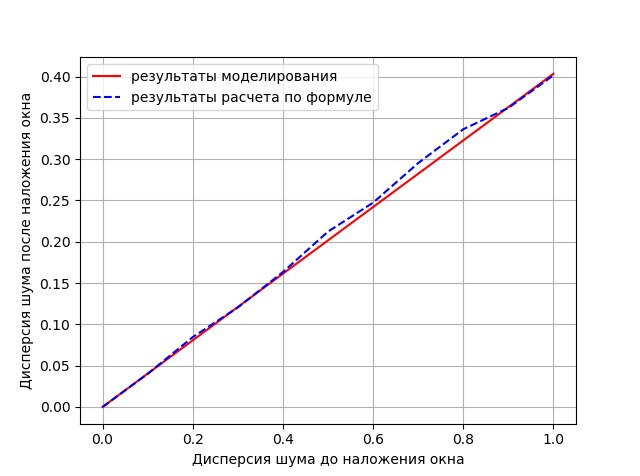
\includegraphics [scale=0.5] {noise_win_var.png}
	\caption{\small{Зависимость дисперсии шума после наложении на него окна.}}
	\label{img:noise_win_var}
\end{figure}

Для рисунка \ref{img:estimate_amp_sin_kaiser_beta} использовалась формула \ref{eq:equation25} для дисперсии оценки амплитуды гармоники при использовании оконной функции. При увеличении числа тестов линии становятся все более похожими. 
\begin{figure}[ht]
	\centering
	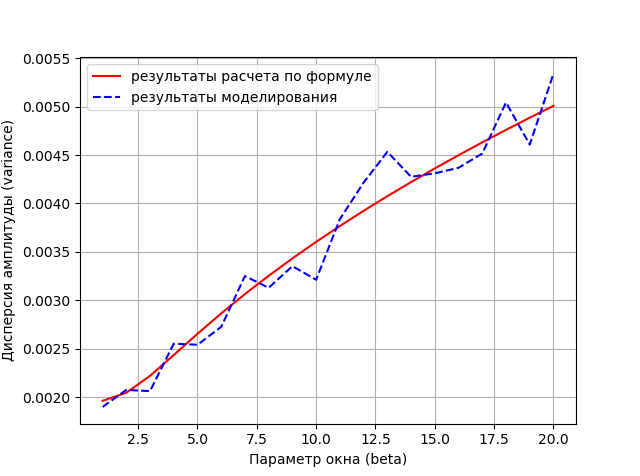
\includegraphics [scale=0.5] {estimate_amp_sin_kaiser_beta.png}
	\caption{\footnotesize{Зависимость дисперсии оценки амплитуды от параметра окна.}}
	\label{img:estimate_amp_sin_kaiser_beta}
\end{figure}

Для рисунка \ref{img:estimate_amp_sin_kaiser_noise} использовалась формула \ref{eq:equation25} для дисперсии оценки амплитуды гармоники при использовании оконной функции.
\begin{figure}[ht]
	\centering
	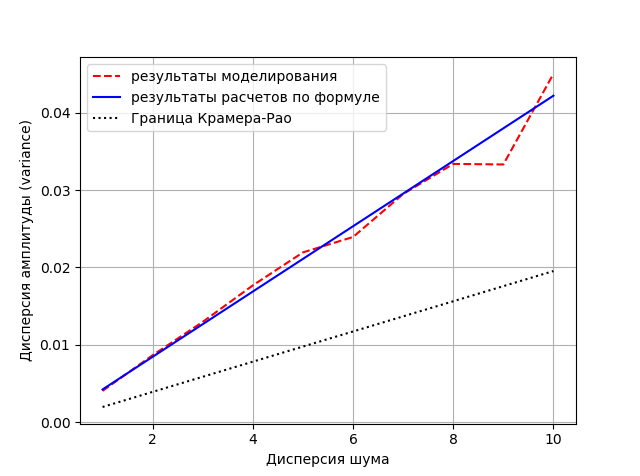
\includegraphics [scale=0.5] {estimate_amp_sin_kaiser_noise.png}
	\caption{\footnotesize{Зависимость дисперсии оценки амплитуды от дисперсии шума.}}
	\label{img:estimate_amp_sin_kaiser_noise}
\end{figure}

Рассмотренили влияние различных оконных функций на границу Крамера-Рао амплитуды однотонального сигнала \cite{altman2020boundary}.
Формула оценки дисперсии амплитуды \cite{altman2020boundary} дает наилучший результаты при выборе весовых функций: Кайзера ($\beta=4$), Хэмминга, Барлетта. Так как результаты расчетов по формуле и результаты моделирование близки к границе Крамера-Рао. Зависимость дисперсии оценки амплитуды от дисперсии шума показывают, что чем меньше коэффициент увеличения дисперсии, тем точнее результаты. Наихудший результат показало окно Кайзера с параметром $\beta=15$.

Исследованы методы оценки спектральных составляющих:
\begin{enumerate}
	\item	Метод Якобсена (Jacobsen's Modified Quadratic Estimator)\cite{4205098, jacobsen1994local, jacobsen2007fast, ericjacobsen_cite};
	\item	Два метода Квина (Quinn's Estimator, Quinn's Second Estimator)\cite{558515, 295186, 330402};
	\item	Два метода Маклеода (Macleod's Estimator) \cite{651200, 1055282};
	\item	Метод Грэндка (Grandke's method) \cite{4315077};
	\item	Алгоритм параболической интерполяции (Parabolic Interpolation) \cite{Konopatskiy_2020, LACHANCE1991143, gasior2004improving, 7818824};
	\item	Алгоритм интерполяции Гаусса (Gaussian Interpolation) \cite{gasior2004improving, gu2005leaf, gilboa2014image};
	\item	Алгоритм, рекомендованный в ГОСТ 30804.4.7-2013 \cite{GOST30804.4.7-2013};
	\item	Метод корреляционных функций (Correlation function method) \cite{Altman2012definition, Altman2012promotion, Altman2012improvement, WANG20175}.
	\item Модернизированный метод корреляционных функций (Modernized method of correlation functions) \cite{Altman2012promotion, Elizarov2016analysis, Increase_Accuracy_Yelizarov2014}.
\end{enumerate}
%B. G. Quinn, "Estimation of frequency, amplitude, and phase from the DFT of a time series," in IEEE Transactions on Signal Processing, vol. 45, no. 3, pp. 814-817, March 1997, doi: 10.1109/78.558515.
% B. G. Quinn, "Estimating frequency by interpolation using Fourier coefficients," in IEEE Transactions on Signal Processing, vol. 42, no. 5, pp. 1264-1268, May 1994, doi: 10.1109/78.295186.
% B. G. Quinn and P. J. Kootsookos, "Threshold behavior of the maximum likelihood estimator of frequency," in IEEE Transactions on Signal Processing, vol. 42, no. 11, pp. 3291-3294, Nov. 1994, doi: 10.1109/78.330402.

% D. Rife and R. Boorstyn, "Single tone parameter estimation from discrete-time observations," in IEEE Transactions on Information Theory, vol. 20, no. 5, pp. 591-598, September 1974, doi: 10.1109/TIT.1974.1055282.
% M. D. Macleod, "Fast nearly ML estimation of the parameters of real or complex single tones or resolved multiple tones," in IEEE Transactions on Signal Processing, vol. 46, no. 1, pp. 141-148, Jan. 1998, doi: 10.1109/78.651200.


%T. Grandke, "Interpolation Algorithms for Discrete Fourier Transforms of Weighted Signals," in IEEE Transactions on Instrumentation and Measurement, vol. 32, no. 2, pp. 350-355, June 1983, doi: 10.1109/TIM.1983.4315077.

%Konopatskiy E. V., Bezditnyi A. A. Geometric modeling of multifactor processes and phenomena by the multidimensional parabolic interpolation method //Journal of Physics: Conference Series. – IOP Publishing, 2020. – Т. 1441. – №. 1. – С. 012063.
% S. Djukanović, T. Popović and A. Mitrović, "Precise sinusoid frequency estimation based on parabolic interpolation," 2016 24th Telecommunications Forum (TELFOR), 2016, pp. 1-4, doi: 10.1109/TELFOR.2016.7818824.


% Gasior M., Gonzalez J. L. Improving FFT frequency measurement resolution by parabolic and Gaussian spectrum interpolation //AIP Conference Proceedings. – American Institute of Physics, 2004. – Т. 732. – №. 1. – С. 276-285.
% Gu X., Du JX., Wang XF. (2005) Leaf Recognition Based on the Combination of Wavelet Transform and Gaussian Interpolation. In: Huang DS., Zhang XP., Huang GB. (eds) Advances in Intelligent Computing. ICIC 2005. Lecture Notes in Computer Science, vol 3644. Springer, Berlin, Heidelberg. https://doi.org/10.1007/11538059_27
% Gilboa E. et al. Image interpolation and denoising for division of focal plane sensors using Gaussian processes //Optics express. – 2014. – Т. 22. – №. 12. – С. 15277-15291.

% Альтман Е. А., Елизаров Д. А. Повышение точности оценки параметров сигналов в электрической сети в системе тягового электроснабжения //Известия Транссиба. – 2012. – №. 3 (11).
% Wang Z. et al. Nonlinearity-tolerant OSNR estimation method based on correlation function and statistical moments //Optical Fiber Technology. – 2017. – Т. 39. – С. 5-11.

% Елизаров Д. А. Анализ методов оценки гармонических составляющих напряжения в электроэнергетических системах //Омский научный вестник. – 2016. – №. 2 (146).

Алгоритмы являются интерполяционными для нахождения параметров гармоник, кроме трех последних методов (метод корреляционных функций, модернизированный метод корреляционных функций и метод по ГОСТу). Сутью метода интерполирования является нахождение промежуточных значений величины по имеющемуся дискретному набору известных значений, то есть кривая построенной функции должна точно пройти через имеющиеся точки данных.

В результате анализа выявлено, что метод корреляционных функций
наиболее точен, но использует большее количество математических операций,
поэтому требует большего времени на выполнение.

\underline{\textbf{Третья глава}} посвящена исследованию численных методов для нахождение оптимальной несмещенной оценки параметров гармоник:

\begin{itemize}
\item Методы, основанные на интерполировании смежных гармоник, позволяют достичь высокой точности, во многих случаях достаточной для практического применения, однако они не позволяют достичь точности оптимальной несмещенной оценки.

\item Можно выделить два подхода к построению алгоритмов на основе корреляционного анализа: использование итерационного процесса для нахождения частоты, амплитуды и фазы каждой гармоники и использование техники дополнения нулями сигнала с целью уплотнения гармоник в спектре сигнала. Оба метода требуют существенно больших вычислительных ресурсов, чем методы основанные на интерполировании, но обеспечивают оптимальную несмещенную оценку.

\item Время расчета параметров гармоник многотонального сигнала с помощью техники дополнения нулями может быть существенно снижено за счет применения разряженного быстрого преобразования Фурье.

\item Реализация итерационного оптимизационного метода нахождения гармоник на основе чисел Фиббоначи при небольшом числе обсчитываемых гармоник обеспечивает быстродействие, близкое к итерационным методам.

\item Реализация метода дополнение нулями сигнала при использовании разряженного преобразования Фурье имеет быстродействие менее чем на порядок худшее, чем итерационные методы, при этом быстродействие не зависит от числа обсчитываемых гармоник. Также нужно отметить больший объем памяти, требуемый для этого метода, который при этом не является критичным для современных вычислительных устройств.
\end{itemize}

Разработан прямой корреляционный метод с использованием быстрых алгоритмов обработки сигналов. Алгоритм поиска гармоник представлен на рисунке \ref{img:Diagram_GSA}:
\begin{figure}[ht]
	\centering
	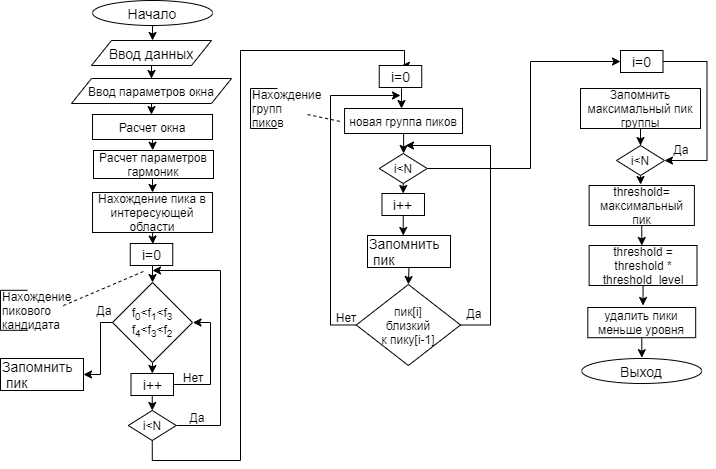
\includegraphics [scale=0.5] {Diagram_GSA2.png}
	\caption{ГСА алгоритма поиска гармоник.}
	\label{img:Diagram_GSA}
\end{figure}

Рассмотрели применение метода разложения двумерной свертки при
реализации цифровых фильтров. Линейная двумерная дискретная свертка определяется следующей формулой \cite{decomposition_method_application2017}:
\begin{equation}
	\label{eq:equation3.5.1}
	CON_{j1,j2} = \sum_{i1 =0}^{n1-1} \sum_{i2 =0}^{n2-1} x_{i1,i2} \cdot y_{i1-j1,i2-j2}
\end{equation} 

Дискретная корреляция двух последовательностей определяется следующей формулой: 
\begin{equation}
	\label{eq:equation3.5.2}
	COR_{j1,j2} = \sum_{i1 =0}^{n1-1} \sum_{i2 =0}^{n2-1} x_{i1,i2} \cdot y_{i1+j1,i2+j2}
\end{equation}

Будем рассматривать три варианта вычисления двумерной свертки. Первый вариант – вычисление двумерной свертки непосредственно по формуле \ref{eq:equation3.5.1}. Второй вариант – использование предложенного в \cite{550562} алгоритма разложения двумерной свертки в несколько двумерных сверток меньших размеров. Третий вариант – использование быстрых алгоритмов одномерной свертки \cite{MOU1987377} для вычисления двумерной свертки.
$$
	CON_{j1,j2} = 
	\begin{bmatrix}
		\left( {B_{j1,j2} + B_{j1,j2+1}} \right) X_{0,0} \\
		\left( {B_{j1+1,j2} + B_{j1+1,j2+1}} \right) X_{1,0} \\
		\left( {B_{j1,j2+1} + B_{j1,j2+2}} \right) X_{0,1} \\
		\left( {B_{j1+1,j2+1} + B_{j1+1,j2+2}} \right) X_{1,1}
	\end{bmatrix}
	+
$$
$$
+
	\begin{bmatrix}
		-1 & 0 \\
		0 & -1 \\
		1 & 0  \\
		0 & 1	
	\end{bmatrix}
	\cdot
	\begin{bmatrix}
		B_{j1,j2+1} \left( {X_{0,0} - X_{0,1}} \right) \\
		B_{j1+1,j2+1} \left( {X_{1,0} - X_{1,1}} \right)	
	\end{bmatrix}
	+
$$
$$
	+ 
	\begin{bmatrix}
		-1 & 0 \\
		1 & 0 \\
		0 & -1  \\
		0 & 1	
	\end{bmatrix}
	\cdot
	\begin{bmatrix}
		\left(	{Y{j1+1,j2} + Y{j1+1,j2+1}} \right) \cdot A_0 \\
		\left(	{Y{j1+1,j2+1} + Y{j1+1,j2+2}} \right) \cdot A_1	
	\end{bmatrix}
	+
$$
\begin{equation}
\label{eq:equation3.5.13}
	+
	\begin{bmatrix}
		1 \\ -1 \\ -1 \\ 1
	\end{bmatrix}
	\cdot
	Y{j1+1,j2+1}
	\cdot
	(A_0 - A_1)
\end{equation}

%Можно сослаться на свои работы в автореферате. Для этого в файле
%\verb!Synopsis/setup.tex! необходимо присвоить положительное значение
%счётчику \verb!\setcounter{usefootcite}{1}!. В таком случае ссылки на
%работы других авторов будут подстрочными.
%Изложенные в третьей главе результаты опубликованы в~\cite{vakbib1, vakbib2}.
%Использование подстрочных ссылок внутри таблиц может вызывать проблемы.

В \underline{\textbf{четвертой главе}} приведено описание применения алгоритмов оценки параметров многотональных сигналов для анализа гармоник и интергармоник в электрических сетях на железнодорожном транспорте:

\begin{itemize}

\item В современных стандартах по анализу спектра в электрических сетях большее внимание уделяется нахождению интергармонических составляющих. Поскольку интергармонические составляющие имеют малую энергию по отношению к другим гармоникам и шуму, к алгоритмам для нахождения параметров гармоник возрастают требования по точности определения амплитуды в условиях высокого шума.

\item В стандартах также указывается требования о нахождение всех гармоник по 40 включительно, что, вместе с требованием о нахождении интеграмоник приводит к большому числу анализируемых гармонических составляющих сигнала.

\item Исходя из требований стандарта и анализа свойств изученных алгоритмов для анализа спектра сигнала в силовых электрических сетях железнодорожного транспорта рекомендуется использование метода дополнения сигнала нулями с применением разряженного преобразования Фурье.

\item Время расчета спектра реального сигнала этим методом на современном компьютере начального уровня составляет единицы секунд, что позволяет говорить о его приемлемом быстродействии для решения практических задач.
\end{itemize}

В четвертом разделе рассматривается понятие качество электрической энергии (КЭ) и описываются стандарты, определяющие состав показателей КЭ и методики измерений. По результатам анализа проводится сравнение российских и иностранных стандартов, описывающих требования и нормы КЭ.

\begin{figure}[ht]
	\centerfloat{
		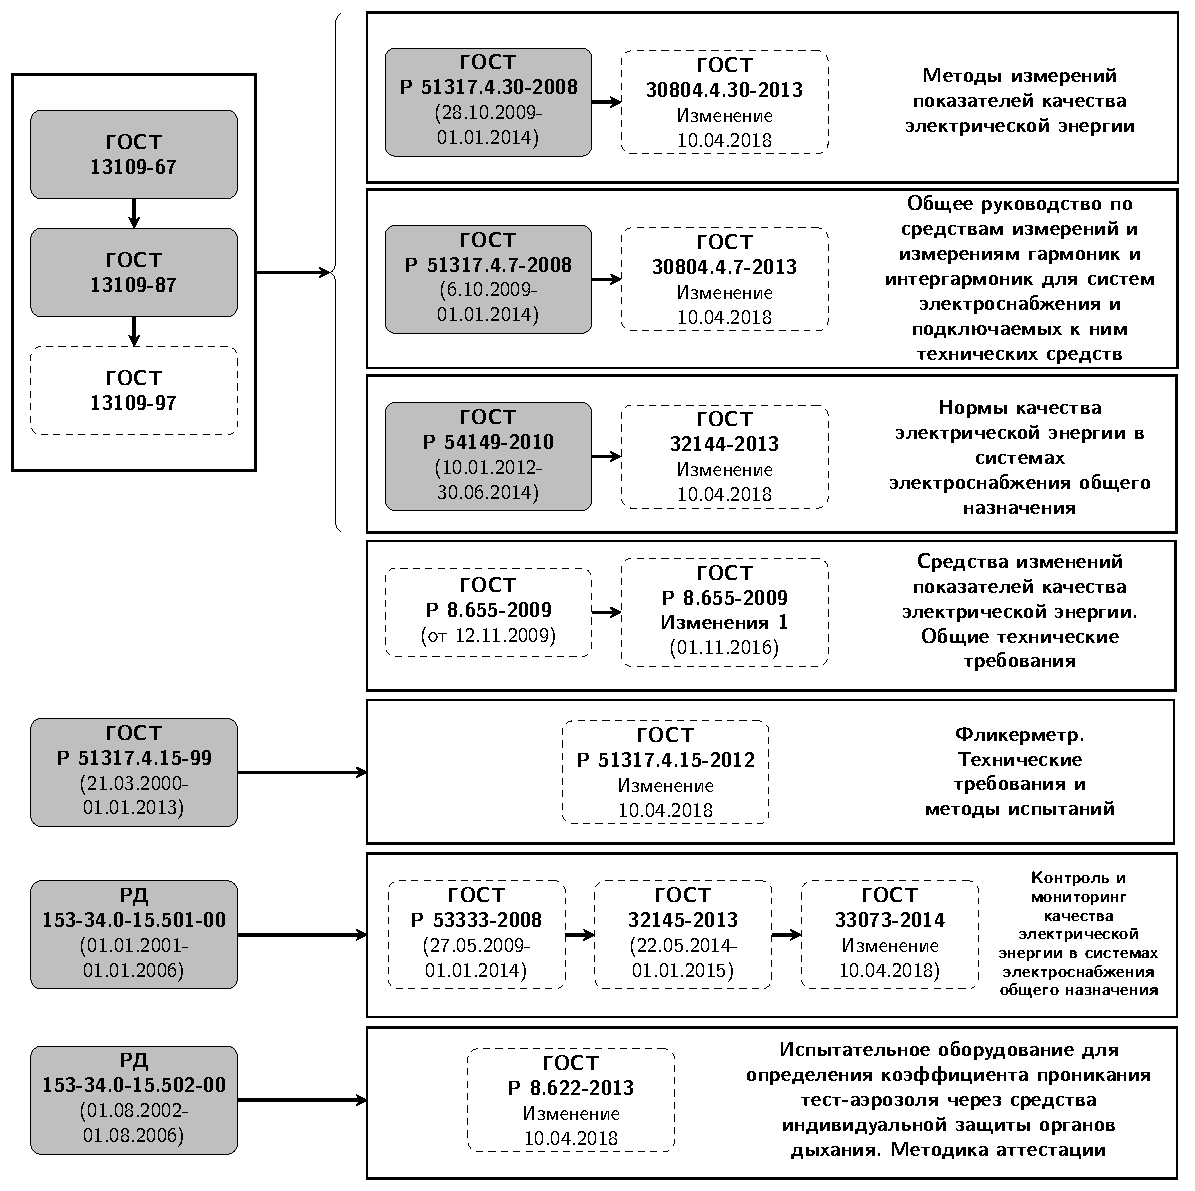
\includegraphics[scale=0.5]{picture1}
	}
	\caption{Развитие государственных стандартов в области контроля КЭ.}\label{img:picture1}
\end{figure} 

В \underline{\textbf{заключении}} приведены основные результаты работы, которые заключаются в следующем:
%% Согласно ГОСТ Р 7.0.11-2011:
%% 5.3.3 В заключении диссертации излагают итоги выполненного исследования, рекомендации, перспективы дальнейшей разработки темы.
%% 9.2.3 В заключении автореферата диссертации излагают итоги данного исследования, рекомендации и перспективы дальнейшей разработки темы.
В результате проведенных исследований получены новые научные результаты и технические решения и разработки, направленные на повышение достоверности, точности и эффективности работы алгоритмов оценивания параметров гармоник.

Их применение позволит обеспечить высокое качество разработки контрольно-измерительных приборов для электрических сетей, а также может быть использованы при создании устройств приема информации для радиосигналов и других систем обработки сигналов.

Основные научные и практические результаты диссертационной работы состоят в следующем:
\begin{enumerate}
  \item Произвели обзор методов: интерпорилрование спектра (метод Якобсена, два метода Квина, два метода Маклеода, метод Грэндка, алгоритм параболической интерполяции, алгоритм интерполяции Гаусса), алгоритм, рекомендованный в ГОСТ $30804.4.7-2013$, метод корреляционныход  функций, Модернизированный метод корреляционных функций, алгоритм вычисления одномерной корреляции, алгоритм вычисления двумерной корреляции, алгоритм дискретного преобразования Фурье (ДПФ), алгоритма быстрого преобразования Фурье (БПФ), алгоритм разряженного преобразования Фурье (Spare FFT). 
  \item Выведена формула для нахождения границы Крамера-Рао при применении оконной функции, которая позволяет повысить эффективность научных исследований различных алгоритмов обработки сигналов с применением оконных функций, заменив моделирование алгоритма с применением различных окон расчетом по предложенной формуле.
  \item Предложенный численный метод, вместе с его быстрой реализацией, позволяют повысить точность и достоверность результатов измерительных приборов для электрических сетей. Численный метод позволяет находить оптимальную несмещенную оценку параметров гармоник.
  \item Разработанный комплекс программ позволяет проводить научные исследования в области цифровой обработки сигналов и используется в учебном процессе: программа прямого корреляционного метода с использование быстрых алгоритмов обработки сигналов, оценка дисперсии белого шума после наложения на него окна, оценка амплитуды при использовании различных окон, оценка амплитуды при различныз уровнях шума, алгоритм вычисления одномерной свертки.
\end{enumerate}

В качестве рекомендаций дальнейшей разработки темы диссертации в части построения математических моделей систем приема и измерения сигналов предлагается распространить подход к определению границы Крамера-Рао для других алгоритмов цифровой обработки сигналов. Перспективным также является изучение и применение разработанных численных методов для оценки гармонических сигналов другого типа, отличного от сигналов в электрической сети.


%При использовании пакета \verb!biblatex! список публикаций автора по теме
%диссертации формируется в разделе <<\publications>>\ файла
%\verb!common/characteristic.tex!  при помощи команды \verb!\nocite!

\ifdefmacro{\microtypesetup}{\microtypesetup{protrusion=false}}{} % не рекомендуется применять пакет микротипографики к автоматически генерируемому списку литературы
\urlstyle{rm}                               % ссылки URL обычным шрифтом
\ifnumequal{\value{bibliosel}}{0}{% Встроенная реализация с загрузкой файла через движок bibtex8
  \renewcommand{\bibname}{\large \bibtitleauthor}
  \nocite{*}
  \insertbiblioauthor           % Подключаем Bib-базы
  %\insertbiblioexternal   % !!! bibtex не умеет работать с несколькими библиографиями !!!
}{% Реализация пакетом biblatex через движок biber
  % Цитирования.
  %  * Порядок перечисления определяет порядок в библиографии (только внутри подраздела, если `\insertbiblioauthorgrouped`).
  %  * Если не соблюдать порядок "как для \printbibliography", нумерация в `\insertbiblioauthor` будет кривой.
  %  * Если цитировать каждый источник отдельной командой --- найти некоторые ошибки будет проще.
  %
  %% authorvak
  \nocite{vakbib1}%
  \nocite{vakbib2}%
  %
  %% authorwos
  \nocite{wosbib1}%
  %
  %% authorscopus
  \nocite{scbib1}%
  %
  %% authorconf
  \nocite{confbib1}%
  \nocite{confbib2}%
  %
  %% authorother
  \nocite{bib1}%
  \nocite{bib2}%

  \ifnumgreater{\value{usefootcite}}{0}{
    \begin{refcontext}[labelprefix={}]
      \ifnum \value{bibgrouped}>0
        \insertbiblioauthorgrouped    % Вывод всех работ автора, сгруппированных по источникам
      \else
        \insertbiblioauthor      % Вывод всех работ автора
      \fi
    \end{refcontext}
  }{
  \ifnum \value{citeexternal}>0
    \begin{refcontext}[labelprefix=A]
      \ifnum \value{bibgrouped}>0
        \insertbiblioauthorgrouped    % Вывод всех работ автора, сгруппированных по источникам
      \else
        \insertbiblioauthor      % Вывод всех работ автора
      \fi
    \end{refcontext}
  \else
    \ifnum \value{bibgrouped}>0
      \insertbiblioauthorgrouped    % Вывод всех работ автора, сгруппированных по источникам
    \else
      \insertbiblioauthor      % Вывод всех работ автора
    \fi
  \fi
  %  \insertbiblioauthorimportant  % Вывод наиболее значимых работ автора (определяется в файле characteristic во второй section)
  \begin{refcontext}[labelprefix={}]    \insertbiblioexternal            % Вывод списка литературы, на которую ссылались в тексте автореферата
  \end{refcontext}
  }
}
\ifdefmacro{\microtypesetup}{\microtypesetup{protrusion=true}}{}
\urlstyle{tt}                               % возвращаем установки шрифта ссылок URL
